\documentclass[xcolor=svgnames]{beamer}
\usepackage[utf8]{inputenc}
\usepackage[english]{babel}

\newcommand{\semitransp}[2][35]{\color{fg!#1}#2}
\usepackage{wrapfig}

\usetheme{Proso}

\title[slepemapy.cz]{Adaptabilní výukový systém pro učení faktických znalostí zeměpisu}
\author{Vít Stanislav}
\institute{Fakulta informatiky Masarykovy univerzity}      % Enter your institute name between curly braces
\date{22. 6. 2015}

\begin{document}
% --------------------------- SLIDE --------------------------------------------
\frame[plain]{\titlepage}
% ------------------------------------------------------------------------------
% --------------------------- SLIDE --------------------------------------------
\begin{frame}
	\frametitle{Procvičování}
   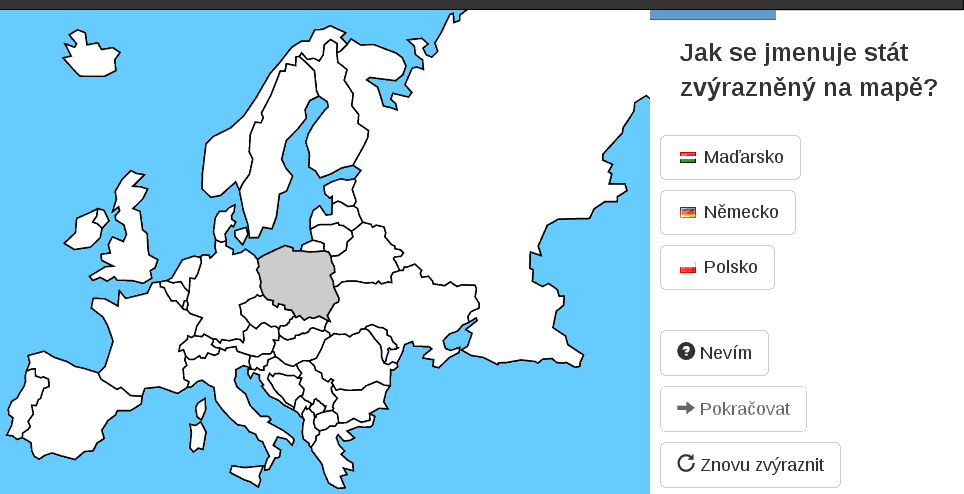
\includegraphics[width=\textwidth]{img/practice-example-cs.png}
\end{frame}
% ------------------------------------------------------------------------------
% --------------------------- SLIDE --------------------------------------------
\begin{frame}
	\frametitle{Mapa znalostí}
   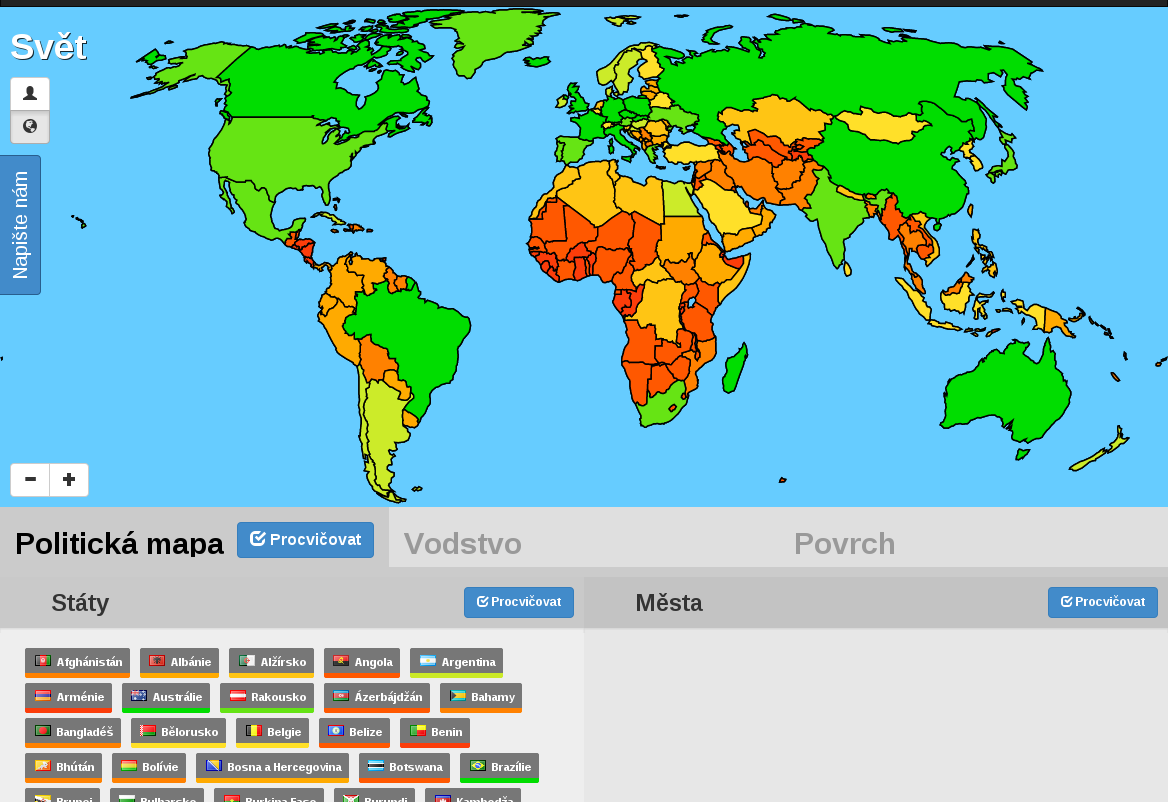
\includegraphics[width=\textwidth]{img/knowledge-map-world.png}
\end{frame}
% ------------------------------------------------------------------------------
% --------------------------- SLIDE --------------------------------------------
\begin{frame}
	\frametitle{Přehled map}
   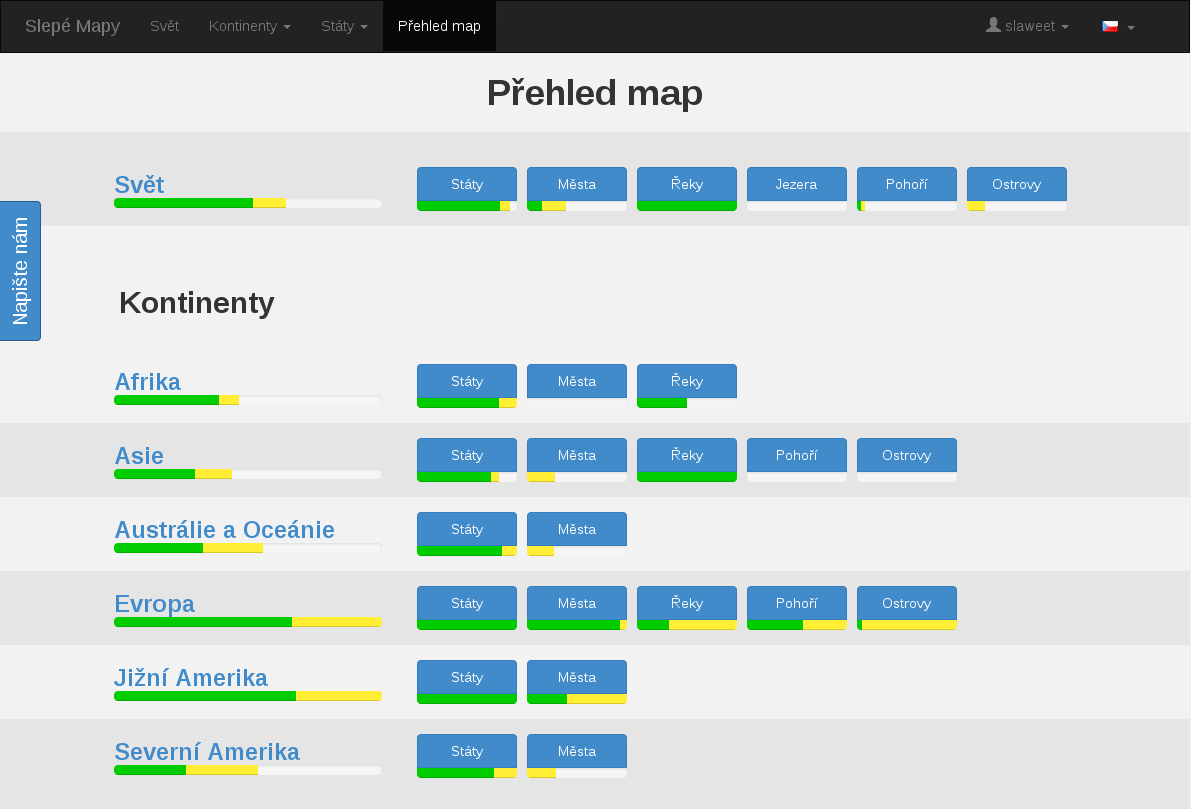
\includegraphics[width=\textwidth]{img/overview.png}
\end{frame}
% ------------------------------------------------------------------------------
% --------------------------- SLIDE --------------------------------------------
\begin{frame}
	\frametitle{Responzivní design}
   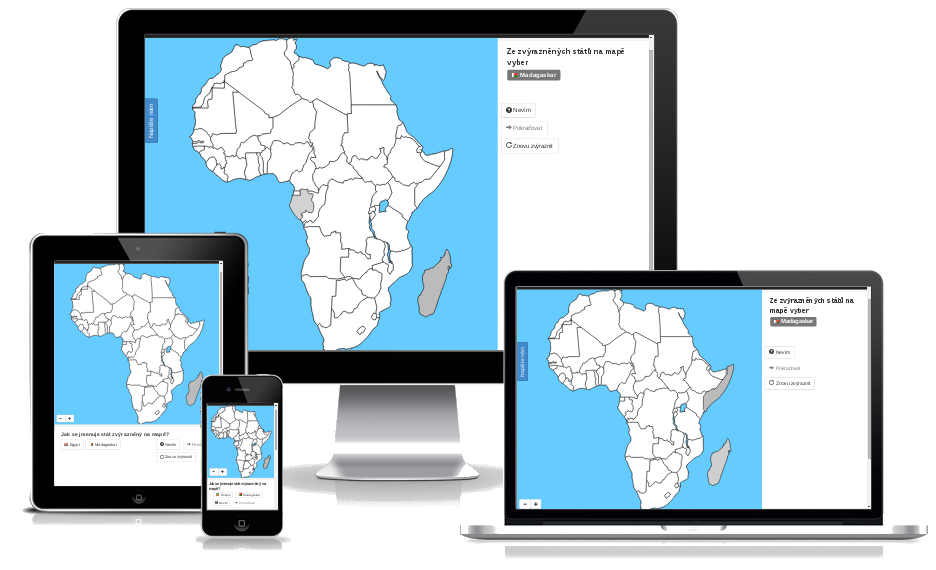
\includegraphics[width=\textwidth]{img/responsive.png}
\end{frame}
% ------------------------------------------------------------------------------
% --------------------------- SLIDE --------------------------------------------
\begin{frame}
	\frametitle{Architektura systému}
   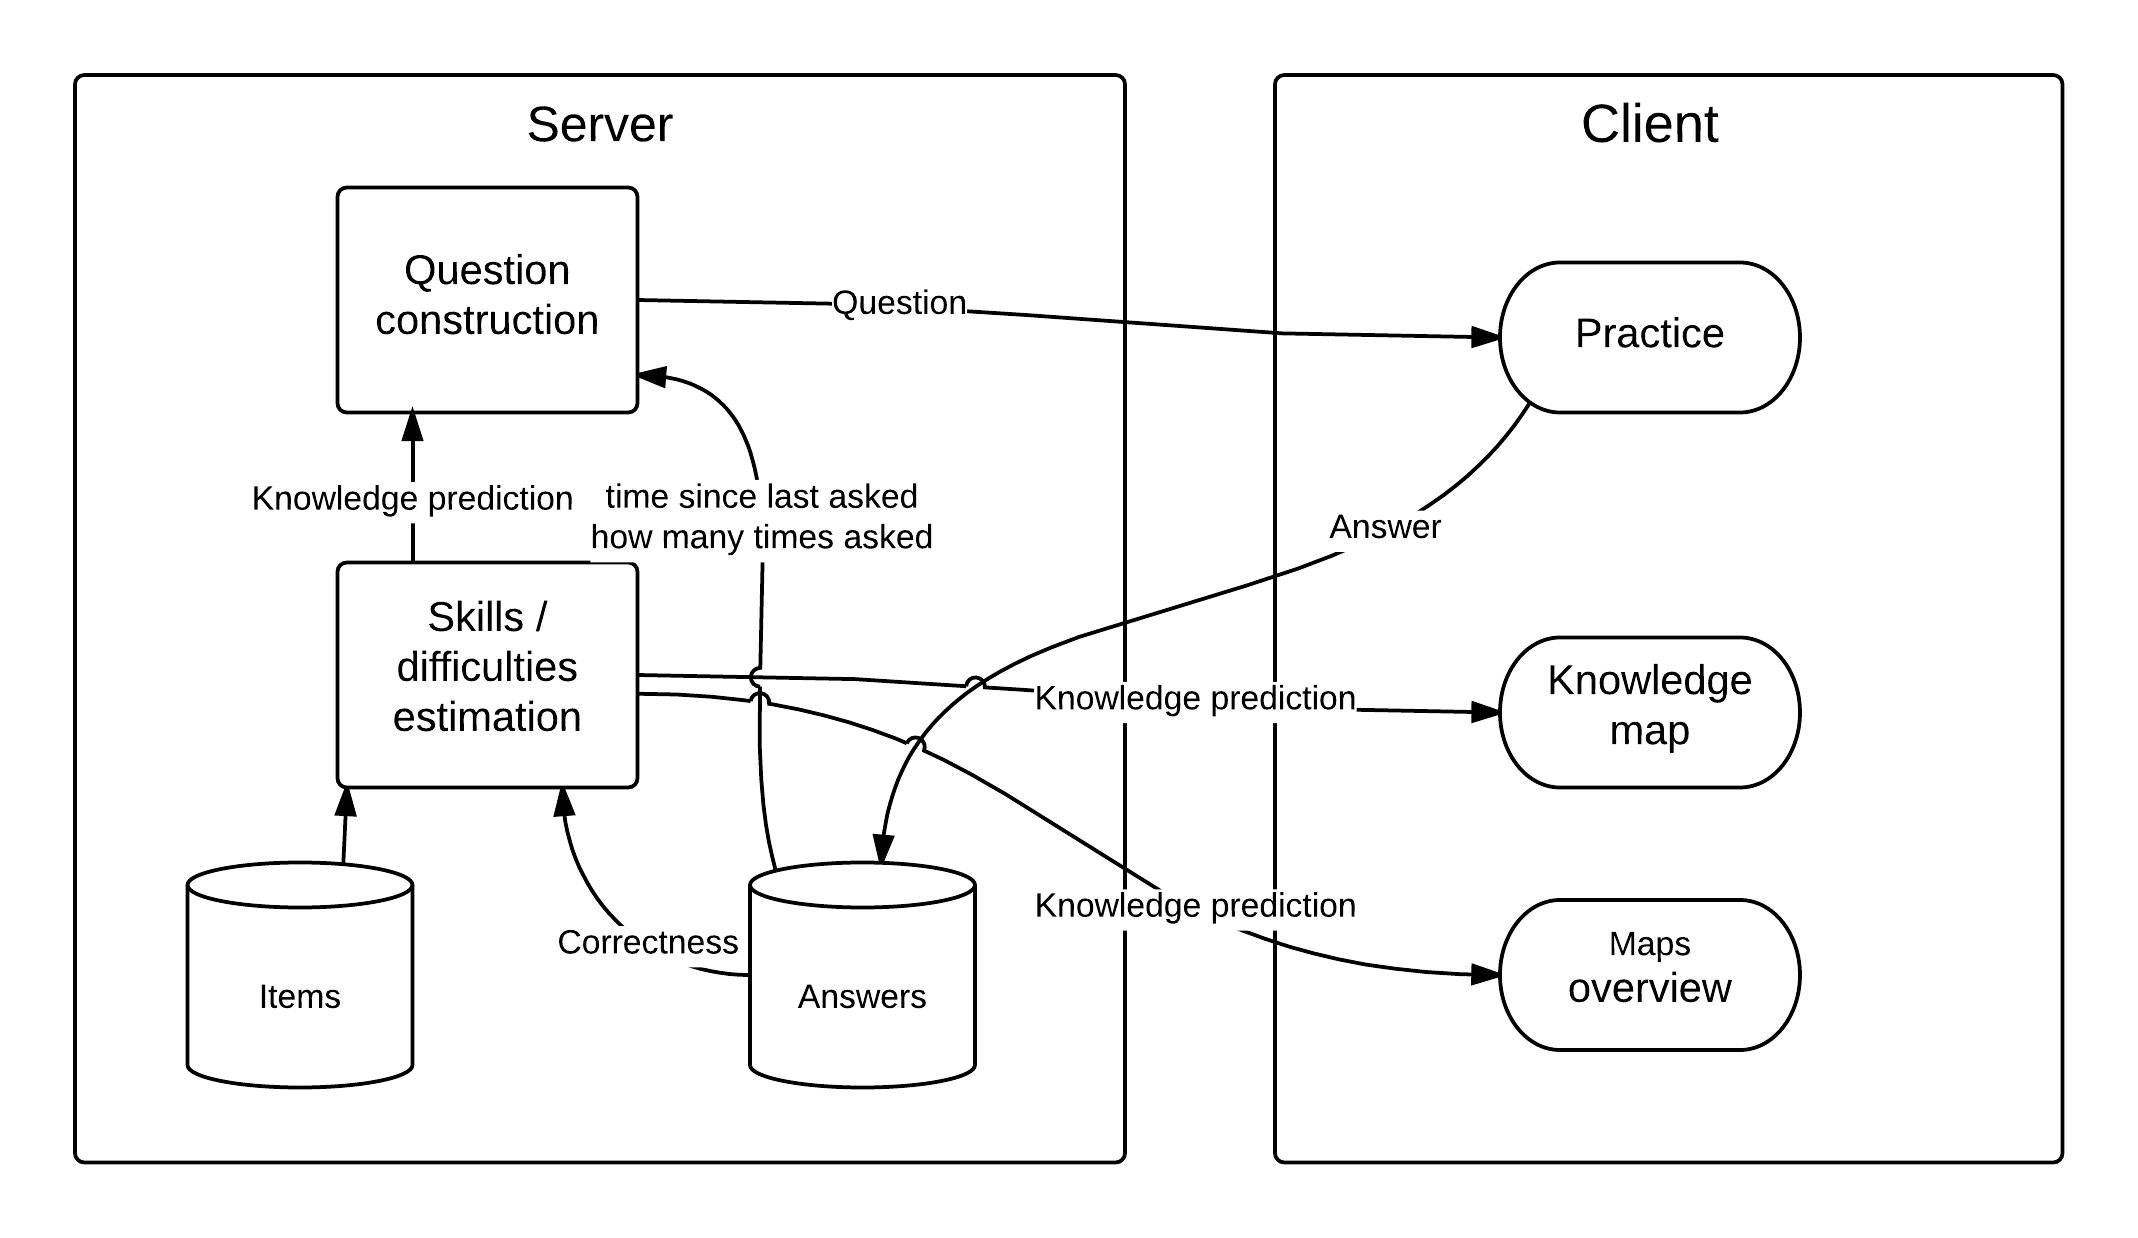
\includegraphics[width=\textwidth]{img/architecture.png}
\end{frame}
% ------------------------------------------------------------------------------
% --------------------------- SLIDE --------------------------------------------
\begin{frame}
	\frametitle{Příprava map}
	\begin{itemize}
    \item Zdroj map: www.NaturalEarthData.com
    \item Zdrojový formát dat: shapefile
    \item kartograph.py $\rightarrow$ SVG
	\end{itemize}
\end{frame}
% ------------------------------------------------------------------------------
% --------------------------- SLIDE --------------------------------------------
\begin{frame}
	\frametitle{Zobrazení map v prohlížeči}
	\begin{itemize}
    \item kartograph.js, Raphaël.js
    \item přiblížení mapy
    \item tooltipy s detaily o položkách
    \
	\end{itemize}
\end{frame}
% ------------------------------------------------------------------------------
% --------------------------- SLIDE --------------------------------------------
\begin{frame}
	\frametitle{Projekt v čase}
     \textbf{Vývoj beta verze} (červen -- listopad 2013)
    \begin{itemize}
      \item procvičování států světa
    \end{itemize}
     \textbf{Studentský projekt na FI} (prosinec 2013 -- květen 2014)
    \begin{itemize}
      \item podpora pro města, řeky, jezera, apod.
      \item přehled map
      \item SEO
    \end{itemize}
     \textbf{Projekt z CTT} (srpen -- prosinec 2014)
    \begin{itemize}
      \item internacionalizace a anglická lokalizace
      \item osobní cíle
      \item anketa obtížnosti otázek
    \end{itemize}
\end{frame}
% ------------------------------------------------------------------------------
% --------------------------- SLIDE --------------------------------------------
\begin{frame}
	\frametitle{Provoz aplikace}
  \begin{itemize}
    \item 200 000 návštěv a 10 milionů odpovědí celkem
    \item 20 000 návštěv a 1 milion odpovědí za poslední měsíc
  \end{itemize}
   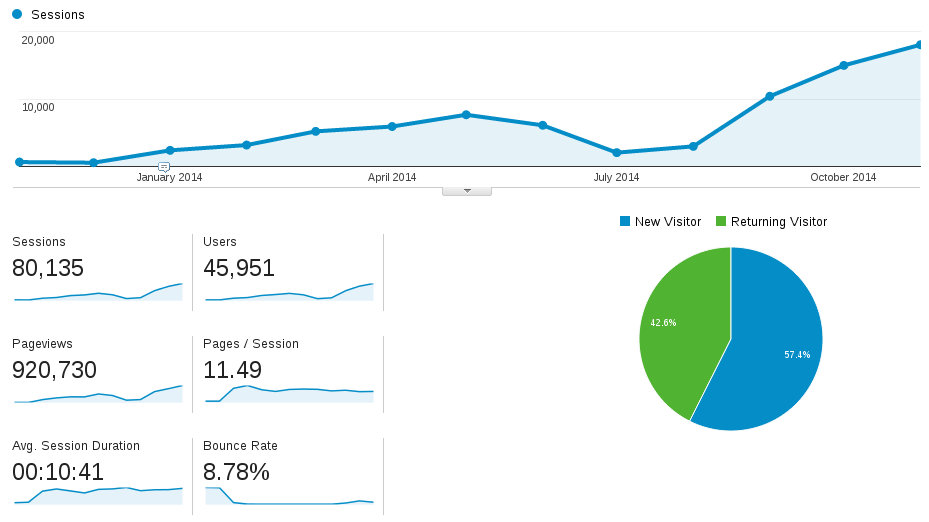
\includegraphics[width=\textwidth]{img/audience.png}
\end{frame}
% ------------------------------------------------------------------------------
% --------------------------- SLIDE --------------------------------------------
\begin{frame}
	\frametitle{Návštěvnost během dne}
   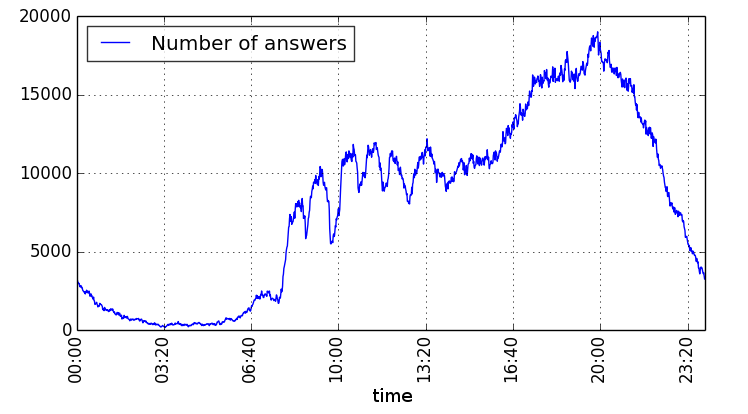
\includegraphics[width=\textwidth]{img/answers_in_day_by_minute_absolute.png}
\end{frame}
% ------------------------------------------------------------------------------
% --------------------------- SLIDE --------------------------------------------
\begin{frame}
	\frametitle{Uživatelé ze škol během dne}
   \includegraphics[width=\textwidth]{img/answers_by_divider_in_day_by_minute_school_divider_20.png}
\end{frame}
% ------------------------------------------------------------------------------
% --------------------------- SLIDE --------------------------------------------
\begin{frame}
	\frametitle{Další analýzy}
   \includegraphics[width=\textwidth]{img/success_by_dividers.png}
\end{frame}
% ------------------------------------------------------------------------------
% --------------------------- SLIDE --------------------------------------------
\begin{frame}
	\frametitle{Zpětná vazba od uživatelů}
   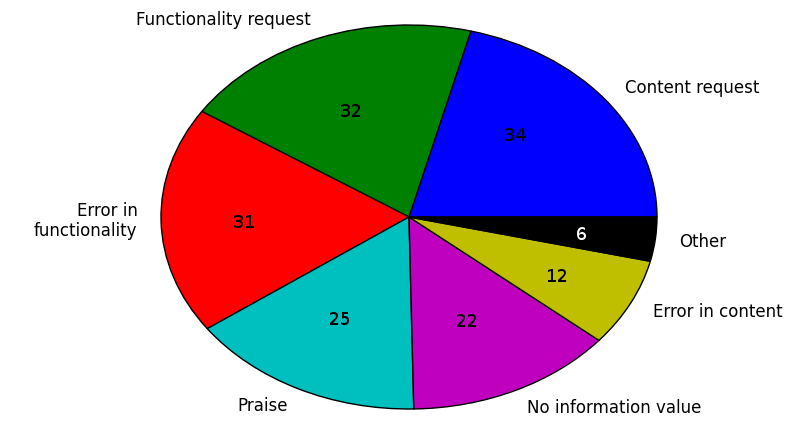
\includegraphics[width=\textwidth]{img/feedback_by_type.png}
\end{frame}
% ------------------------------------------------------------------------------
% --------------------------- SLIDE --------------------------------------------
\begin{frame}
	\frametitle{autoskolachytre.cz}
	 
   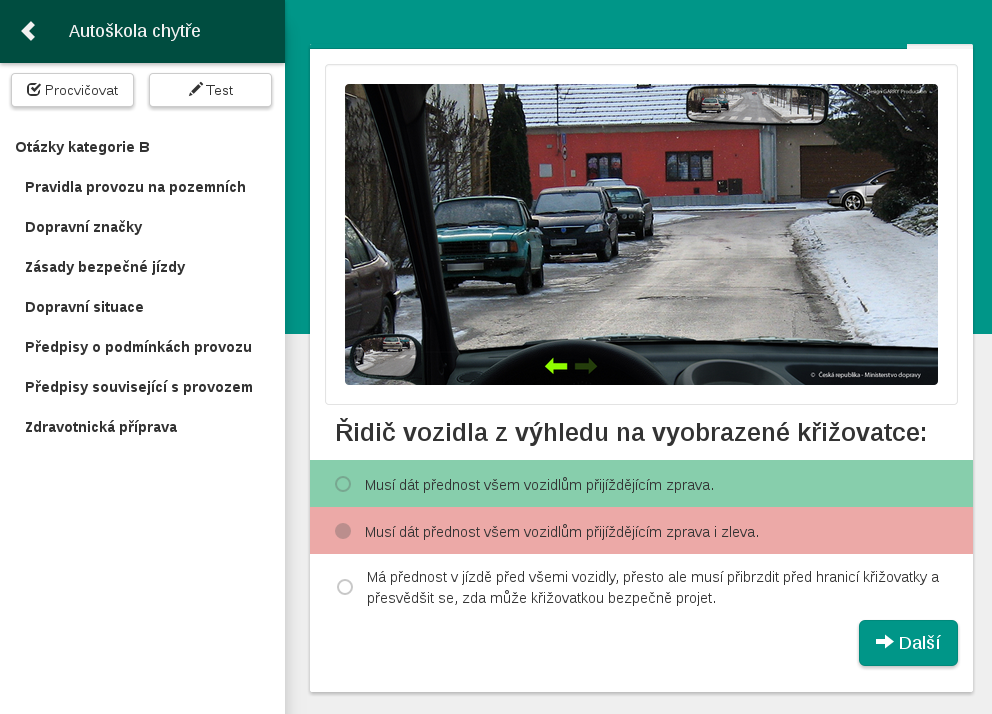
\includegraphics[width=\textwidth]{img/autoskola.png}
\end{frame}
% ------------------------------------------------------------------------------
% --------------------------- SLIDE --------------------------------------------
\begin{frame}
	\frametitle{anatom.cz}
	 
   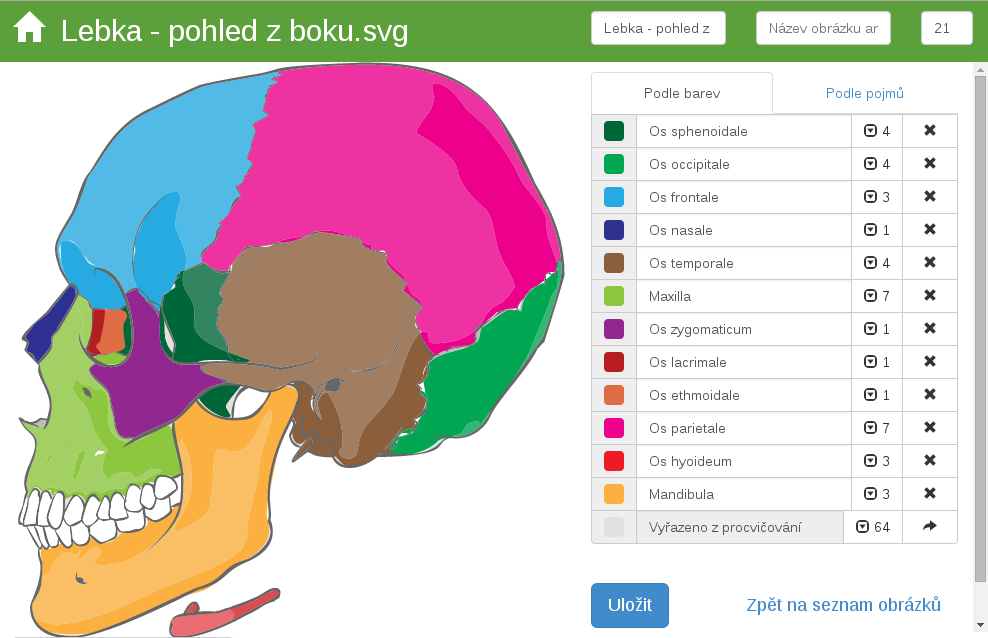
\includegraphics[width=\textwidth]{img/anatomie.png}
\end{frame}
% ------------------------------------------------------------------------------
% --------------------------- SLIDE --------------------------------------------
\begin{frame}
	\frametitle{Výzkum na posbíraných datech}

  \begin{itemize}
   \item \textbf{Adaptabilní procvičování}

  \begin{itemize}
   \item J. Papoušek, R. Pelánek, \textbf{V. Stanislav}. Adaptive Practice of Facts in Domains with Varied Prior Knowledge. Educational Data Mining (EDM), 2014.
   \item J. Papoušek, R. Pelánek. Impact of Adaptive Educational System Behaviour on Student Motivation. Artificial Intelligence in Education (AIED), 2015.
   \item J. Papoušek, R. Pelánek, J. Řihák, \textbf{V. Stanislav}. An Analysis of Response Times in Adaptive Practice of Geography Facts. Educational Data Mining (EDM), 2015.
  \end{itemize}

   \item \textbf{Modelování studentů }

  \begin{itemize}
   \item J. Nižnan, R. Pelánek, J. Řihák. Student Models for Prior Knowledge Estimation. Educational Data Mining (EDM), 2015.
   \item R. Pelánek. Modeling Students' Memory for Application in Adaptive Educational Systems. Educational Data Mining (EDM), 2015.
  \end{itemize}
  \end{itemize}

\end{frame}
% ------------------------------------------------------------------------------
% --------------------------- SLIDE --------------------------------------------
\begin{frame}
	\frametitle{Další závěrečné práce}
  \begin{itemize}
  \item Dionýz Lazar - Analýza dat ze systému pro výuku zeměpisu (bakalářská práce)
  \item Jan Kučera - Adaptabilní webový systém pro výuku anatomie, slepaanatomie.cz (diplomová práce)
  \end{itemize}
\end{frame}
% ------------------------------------------------------------------------------
% --------------------------- SLIDE --------------------------------------------
\begin{frame}
  \frametitle{~}
\begin{center} 
\huge  Děkuji za pozornost.
\end{center}
\end{frame}
% ------------------------------------------------------------------------------
\end{document}
